\chapter{Geometry and analysis: distance, dimension, and complex structure}
\label{learn:geometry}

\begin{learningcard}{Prerequisites and scope}
Bring real limits and derivatives from Chapter~\ref{learn:calculus}, partial
derivatives from Chapter~\ref{learn:multivariable}, and complex arithmetic
from precalculus. Three questions guide this chapter: what does ``nearby''
mean, how can a set have fractional dimension, and what extra structure makes
a complex function modular? These are entrances to topology, fractal geometry,
and complex analysis, with a worked example at each entrance.
\end{learningcard}

\section{Distance comes with axioms}
A metric on a set $X$ is a function $d:X\times X\to\RR$ satisfying
$d(x,y)\geq0$, equality exactly when $x=y$, symmetry
$d(x,y)=d(y,x)$, and the triangle inequality
$d(x,z)\leq d(x,y)+d(y,z)$. Euclidean distance is an example. On $\RR^2$,
the Manhattan distance $|x_1-y_1|+|x_2-y_2|$ is another, useful when
horizontal and vertical travel supply the permitted paths.

The open ball $B_r(x)$ consists of points whose distance from $x$ is less
than $r$. A subset is open when every one of its points has an open ball
contained in the subset. Open sets record which perturbations stay inside
a region. A topology generalizes these neighborhood relations through a
collection of open sets, even when a preferred metric is absent.

A set is compact when every cover by open sets admits a finite subcover.
In Euclidean space, compactness is equivalent to being closed and bounded.
This equivalence is special to finite-dimensional Euclidean space and related
settings, rather than a definition valid in every metric space. A continuous
real function on a nonempty compact set attains its maximum and minimum.
This is the analysis input used in the symmetric spectral theorem of
Chapter~\ref{learn:linear_algebra}.

\section{Worked example: why an excluded endpoint matters}
On the closed interval $[0,1]$, the continuous function $f(x)=x$ attains
its maximum one. On the open interval $(0,1)$, it is bounded above by one
but has no maximum: for every proposed maximizing point $x$, the point
$(x+1)/2$ lies in the interval and has a larger function value.
The same formula has different extremum behavior because the domain changed.

The interval $(0,1)$ also has the open cover
$\{(1/n,1):n\geq2\}$, interpreted as open subsets of $(0,1)$.
Every point is covered by choosing $n>1/x$. A finite selection has a
largest index $N$ and leaves points at or below $1/N$ uncovered.
The failure of compactness is visible through the definition itself.

\section{Worked example: count scales in the Cantor set}
Start with $[0,1]$, remove the open middle third, then repeat the removal
inside every surviving interval. The middle-thirds Cantor set $C$ is the
intersection of all stages. Stage $n$ contains $2^n$ closed intervals of
length $3^{-n}$. If $N(\epsilon)$ is the least number of intervals of
length at most $\epsilon$ needed to cover $C$, then at these scales
$N(3^{-n})=2^n$. The stage intervals supply a cover; selecting their
left endpoints supplies $2^n$ points mutually farther apart than $3^{-n}$,
so a shorter cover needs at least that many intervals.

\begin{figure}[htbp]
  \centering
  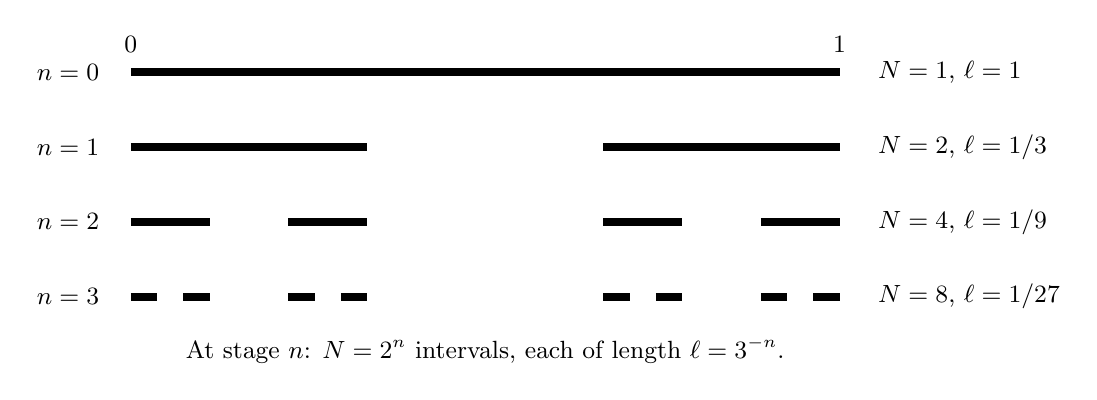
\begin{tikzpicture}[x=9cm,y=0.95cm,font=\small,line width=0.8pt]
  \foreach \stage in {0,1,2,3} {
    \node[left] at (-0.03,-\stage) {$n=\stage$};
  }
  \draw[line width=3pt] (0,0)--(1,0);
  \foreach \numerator in {0,2} {
    \draw[line width=3pt] ({\numerator/3},-1)--({(\numerator+1)/3},-1);
  }
  \foreach \numerator in {0,2,6,8} {
    \draw[line width=3pt] ({\numerator/9},-2)--({(\numerator+1)/9},-2);
  }
  \foreach \numerator in {0,2,6,8,18,20,24,26} {
    \draw[line width=3pt] ({\numerator/27},-3)--({(\numerator+1)/27},-3);
  }
  \node[above] at (0,0.12) {$0$};
  \node[above] at (1,0.12) {$1$};
  \node[right] at (1.04,0) {$N=1$, $\ell=1$};
  \node[right] at (1.04,-1) {$N=2$, $\ell=1/3$};
  \node[right] at (1.04,-2) {$N=4$, $\ell=1/9$};
  \node[right] at (1.04,-3) {$N=8$, $\ell=1/27$};
  \node[below] at (0.5,-3.4) {At stage $n$: $N=2^n$ intervals, each of length $\ell=3^{-n}$.};
\end{tikzpicture}

  \caption{Read downward from the whole interval to successive removals. Each surviving interval produces two intervals one third as long. The right-hand labels record the count and individual length whose logarithmic ratio gives the dimension.}
  \label{fig:learn:cantor_construction}
\end{figure}

When the limit exists, box dimension is
\[
 \dim_B C=\lim_{\epsilon\to0}
 \frac{\log N(\epsilon)}{\log(1/\epsilon)}.
\]
At stage scales the ratio is $\log2/\log3$. For intermediate scales,
monotonicity traps covering counts between neighboring stage counts, giving
the same limit. Thus $\dim_B C=\log2/\log3\approx0.63093$.

Hausdorff dimension instead permits covers with different small diameters.
For $s\geq0$, minimize $\sum_j(\operatorname{diam}U_j)^s$ over countable
covers with diameters at most $\delta$, then let $\delta\to0$ to define
Hausdorff $s$-measure. The dimension is the threshold above which that
measure is zero. The Cantor stage cover has cost
$2^n(3^{-n})^s=(2\,3^{-s})^n$, proving the upper bound
$\dim_H C\leq\log2/\log3$.

For the matching lower bound, assign mass $2^{-n}$ to each stage-$n$
interval. These consistent assignments define the uniform Cantor probability
measure. An interval of length $\ell$, where
$3^{-n}\leq\ell<3^{-(n-1)}$, meets at most four stage-$n$ intervals.
Its mass is therefore at most $4\,2^{-n}\leq4\ell^s$ for
$s=\log2/\log3$. Any small cover of $C$ consequently has
$1\leq4\sum_j(\operatorname{diam}U_j)^s$, by containing each covering
set in an interval of its diameter. The Hausdorff $s$-measure is positive,
proving the lower bound. The two dimensions agree for this set; other sets
can separate them \citep{falconer2004fractal}.

\begin{learningcard}{Historical situation: a measurement question changes with scale}
Mandelbrot's 1967 paper asks how long Britain's coast is and relates
scale-dependent length measurements to statistical self-similarity and
fractional dimension \citep{mandelbrot1967long}. The publication supplies a
specific historical example of a measurement problem motivating geometric
language. An actual coastline has material and observational scale limits;
the exact Cantor construction is a mathematical model with indefinitely
repeated structure. A finite log--log fit to data estimates behavior over
its fitted scales rather than proving an asymptotic dimension.
\end{learningcard}

\section{Complex differentiation controls every approach direction}
For $z=x+iy$, a complex derivative is the limit
$f'(z)=\lim_{h\to0}[f(z+h)-f(z)]/h$ with complex $h$ approaching zero
from all directions. Write $f=u+iv$. Approaching along the real and imaginary
axes gives the necessary Cauchy--Riemann equations
\[
 u_x=v_y,\qquad u_y=-v_x.
\]
If the real partial derivatives are continuous in a neighborhood and satisfy
these equations there, the function is complex differentiable there. A
function complex differentiable throughout an open region is holomorphic.

For $f(z)=z^2$, $u=x^2-y^2$ and $v=2xy$ satisfy the equations, and
expanding $(z+h)^2$ gives $f'(z)=2z$. For $f(z)=\overline z$,
the real-axis difference quotient is one and the imaginary-axis quotient
is minus one, so the complex derivative fails everywhere. A real
coordinate formula alone therefore says little about holomorphy.

\section{Modular forms need a boundary condition too}
Let $\mathcal H=\{\tau\in\CC:\operatorname{Im}\tau>0\}$.
Integer matrices with determinant one form $\mathrm{SL}(2,\ZZ)$ and act by
$\tau\mapsto(a\tau+b)/(c\tau+d)$. Direct algebra gives
\[
 \operatorname{Im}\frac{a\tau+b}{c\tau+d}
 =\frac{\operatorname{Im}\tau}{|c\tau+d|^2}>0.
\]
Two basic transformations are $T(\tau)=\tau+1$ and $S(\tau)=-1/\tau$.
At $\tau=i$, $S(i)=i$ while $T(i)=1+i$; both stay in $\mathcal H$.

A modular form of integer weight $k$ for the full modular group is a
holomorphic function on $\mathcal H$ satisfying
$f((a\tau+b)/(c\tau+d))=(c\tau+d)^k f(\tau)$ and holomorphic at
the cusp. For this group the cusp condition means that its expansion in
$q=e^{2\pi i\tau}$ near $q=0$ has only nonnegative powers.
For subgroups, every inequivalent cusp must be checked. A cusp form has
zero constant term at each cusp. These conditions distinguish a modular
form from a function that merely obeys a transformation law
\citep{diamond2005first}. The invariant $j$, whose expansion starts with
$q^{-1}$, has a pole at the cusp and is a modular function, not a
holomorphic modular form there. Classification and coefficient theorems
require a further course in complex analysis and modular forms.

\section{Exercises with full solutions}
\paragraph{1. Compare two metrics.}
Find the Euclidean and Manhattan distances between $(0,0)$ and $(3,4)$.

\paragraph{Solution.}
Euclidean distance is $\sqrt{3^2+4^2}=5$. Manhattan distance is
$|3|+|4|=7$. Both obey metric axioms, but they encode different path costs.
The pair of values demonstrates that choosing a metric is substantive.

\paragraph{2. Recover a scaling exponent.}
A separated self-similar construction keeps four pieces, each scaled by
$1/5$. Find its similarity dimension, and state the needed qualification.

\paragraph{Solution.}
The scaling equation is $4(1/5)^s=1$, giving $s=\log4/\log5$.
For similarities satisfying an appropriate separation condition, such as
the open set condition, this exponent equals Hausdorff dimension. Without
such a condition, overlapping pieces can invalidate the inference.

\paragraph{3. Use a modular transformation at a fixed point.}
If $f$ has weight two for the full modular group, what does $S(i)=i$
force about $f(i)$?

\paragraph{Solution.}
The transformation law for $S$ gives $f(-1/\tau)=\tau^2 f(\tau)$.
At $i$, it becomes $f(i)=i^2f(i)=-f(i)$, hence $f(i)=0$.
This is a necessary consequence of the transformation law; it alone
constructs neither a nonzero form nor its coefficients.
